\documentclass{article}
\usepackage[utf8]{inputenc}
\usepackage{graphicx}
\usepackage{subfigure}
\usepackage{float}
\usepackage{indentfirst}
\usepackage{caption}
\usepackage{subcaption}
\usepackage[a4paper,includeheadfoot,margin=3cm]{geometry}
\usepackage{amsmath}
\usepackage[subrefformat=parens,labelformat=parens]{subfig}
%\titleformat{\subsection}{\normalsize}%{}{0em}{}

\title{DD2423 - Image Analysis and Computer Vision\\
  \large Lab 3}
\author{
  Gabriela Zarzar Gandler\\
  \texttt{gzrsm@kth.se}
  \and
 Huijie Wang\\
  \texttt{huijiew@kth.se}
}
\date{December 2016}


\begin{document}

\maketitle

\begin{enumerate}
\addtocounter{section}{1}
\section{K-means clustering}
    
    %Disadvantages of K-means: Initial conditions + determining K
    
    \item %Q1
    \textbf{How did you initialize the clustering process and why do you believe this was a good method of doing it?}
    \par
    
    We initialize the clusters by picking $K$ random pixel values in the image. We compared this method with picking $K$ random colors in the RGB space. We believe the first approach is more effective, because it avoids picking values that are too far from the values in the image.
    
    The result is shown as Figure \ref{fig:q1}:
    \begin{figure}[H]
        \centering
        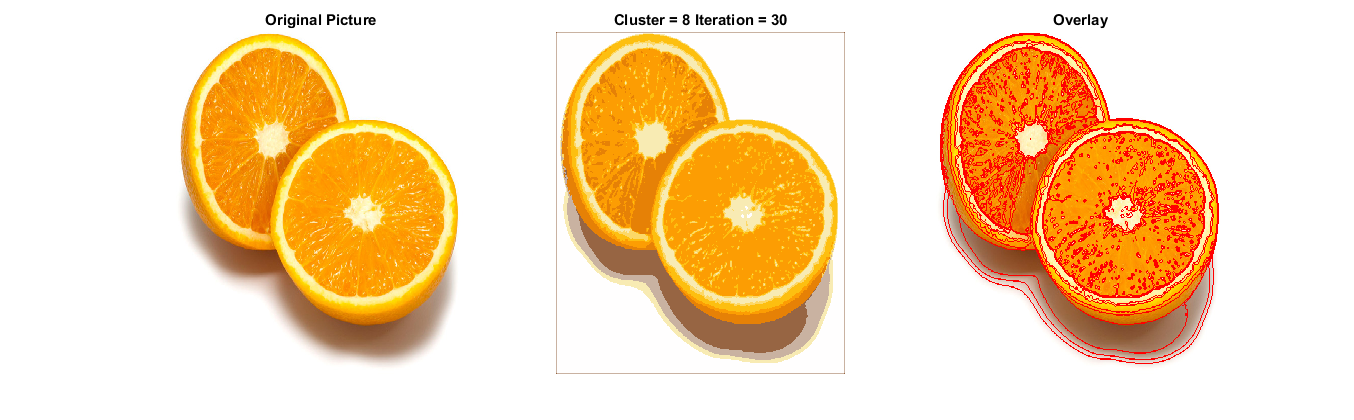
\includegraphics[width=\linewidth]{kmeans_r.png}
        \caption{Result of K-means}
        \label{fig:q1}
    \end{figure}
    \par
    
    \item %Q2
    \textbf{How many iterations L do you typically need to reach convergence, that is the point where no additional iterations will affect the end results?}
    \par
    For $K = 8$, between 49 and 88 iterations are necessary. But it is noticeable that the centers changes very little after iteration = 10. For $K = 16$, between 107 and 156 iterations are necessary. The fewer clusters, the shorter the convergence time. In order to measure the number of iterations until convergence, we check if the centers of the clusters are the same between one iteration and the other.

    \item %Q3
    \textbf{What is the minimum value for K that you can use and still get no superpixel that covers parts from both halves of the orange?}
    \par
    
    It is hard to find an optimal $K$ for this. $K = 18$ still doesn't offer an optimal segmentation. This was expected, because the colors are not reliable criteria to segment the halves of the oranges.
    \begin{figure}[H]
        \centering
        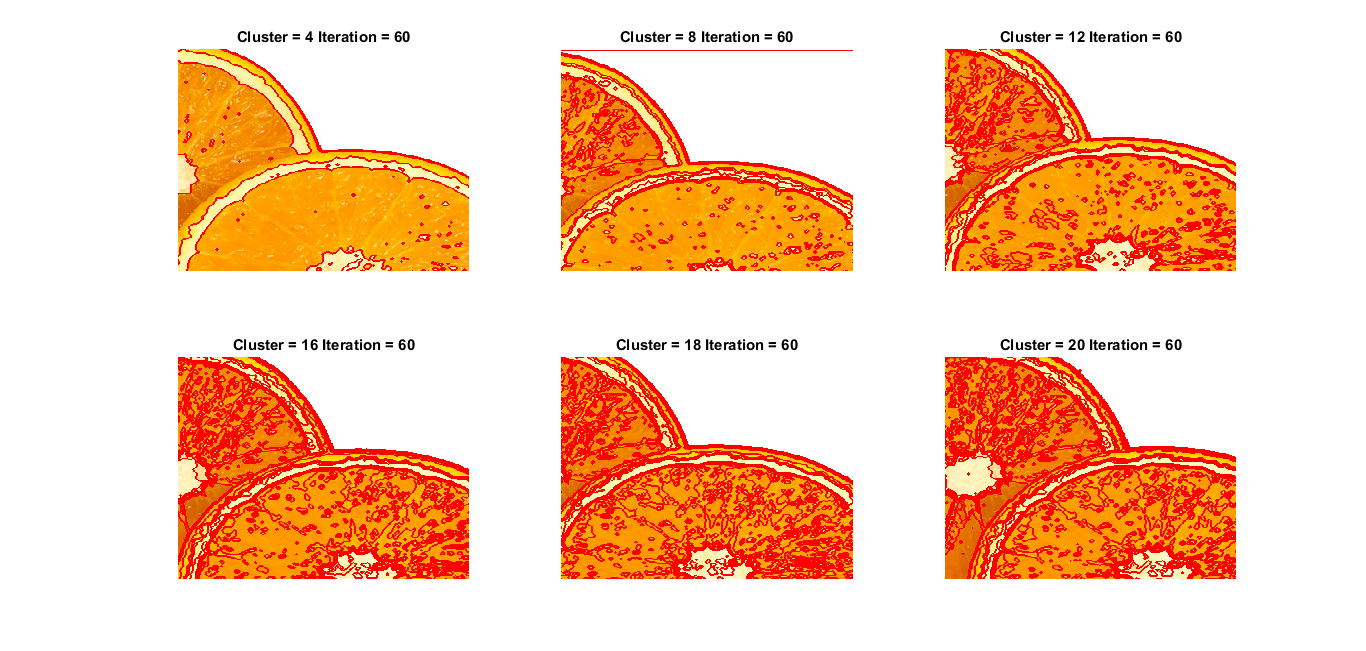
\includegraphics[width=1.2\linewidth]{superpixel.png}
        \caption{Test on superpixels}
        \label{fig:3}
    \end{figure}
    
    \item %Q4
    \textbf{What needs to be changed in the parameters to get suitable superpixels for the tiger images as well?}
    \par
    Parameter K should be changed and L should be set to suitable size.
    The results are shown as Figure \ref{fig:4-01}, \ref{fig:4-02} and \ref{fig:4-03}.

    \begin{figure}[H]
        \centering
        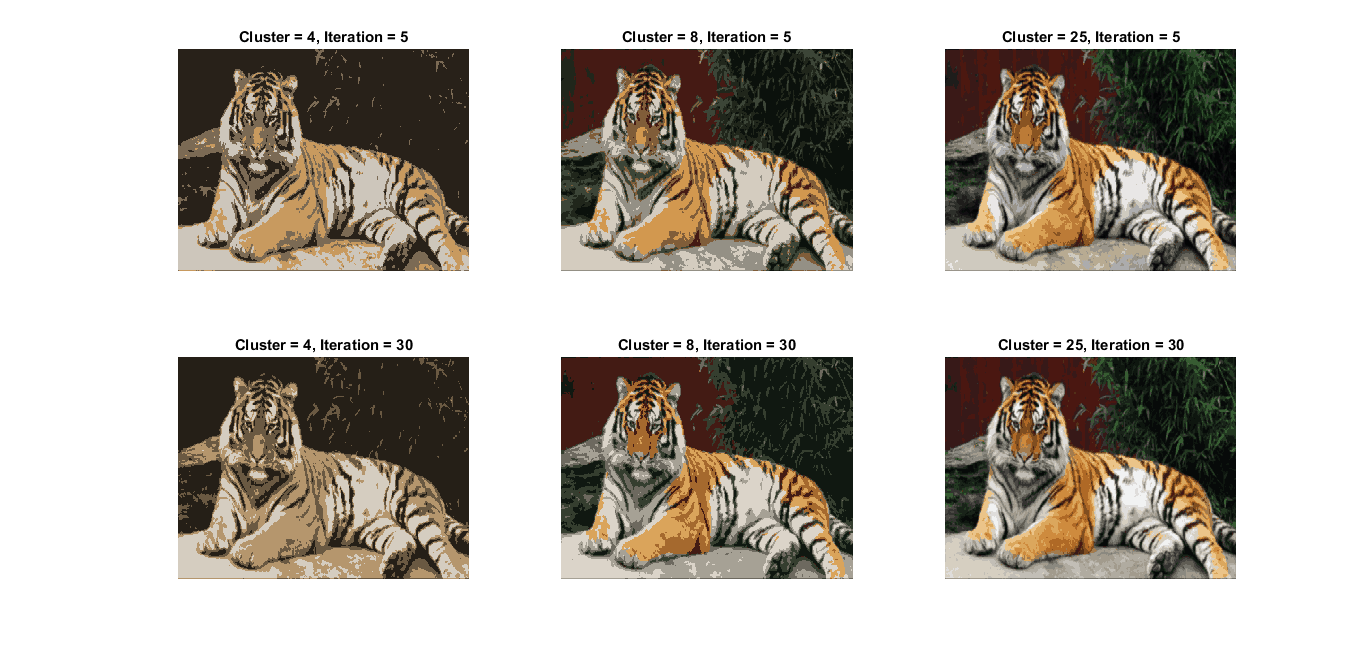
\includegraphics[width=\linewidth]{kmeans_para1.png}
        \caption{Result of  \textit{tiger1.jpg}}
        \label{fig:4-01}
    \end{figure}

    \begin{figure}[H]
        \centering
        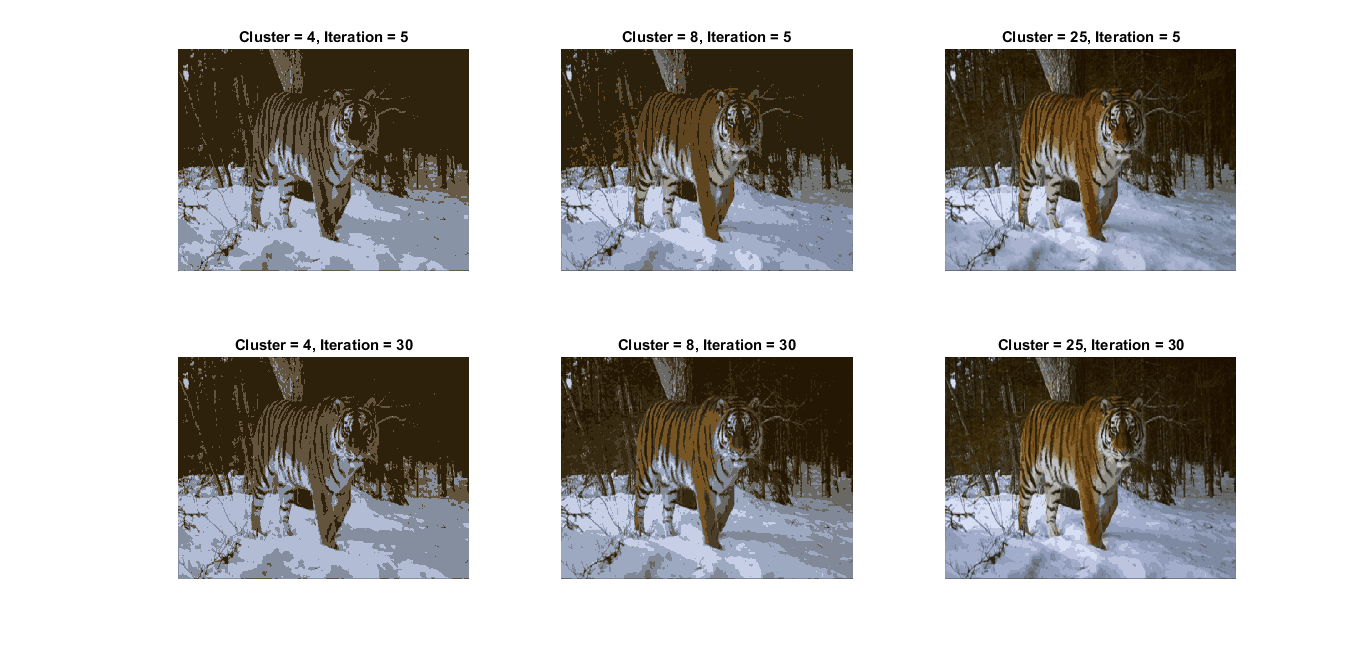
\includegraphics[width=\linewidth]{kmeans_para2.png}
        \caption{Result of \textit{tiger2.jpg}}
        \label{fig:4-02}
    \end{figure}

    \begin{figure}[H]
        \centering
        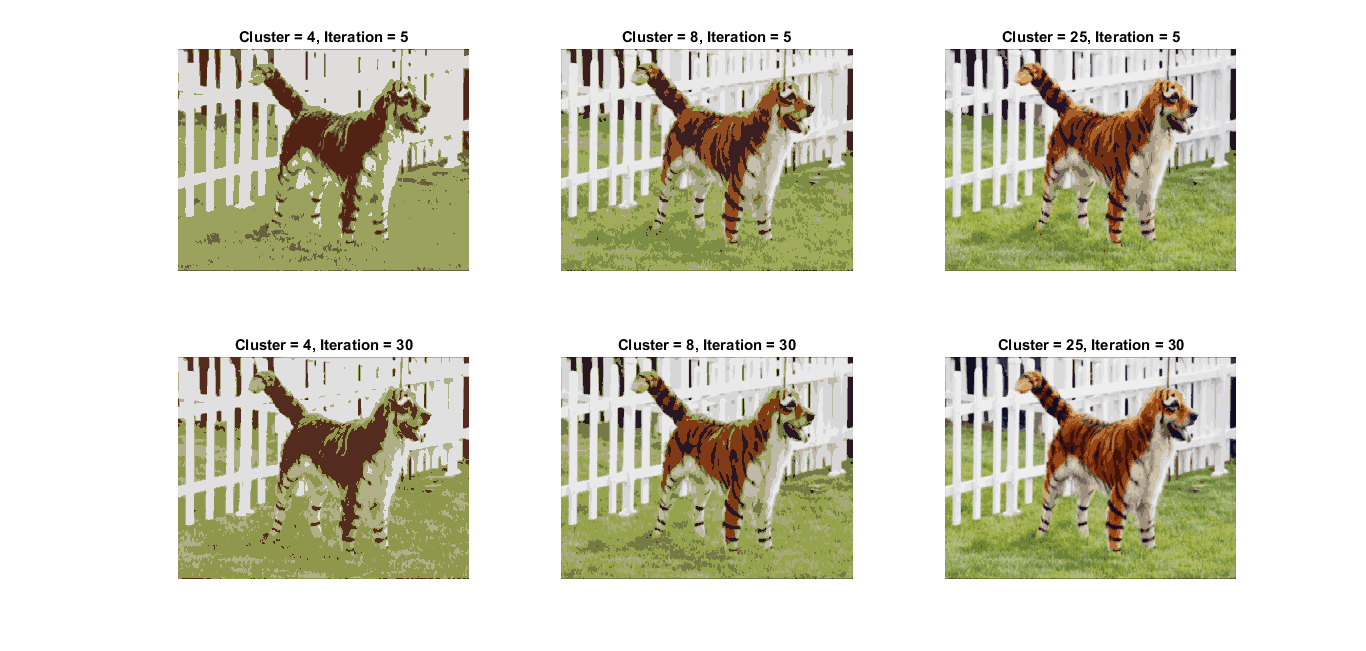
\includegraphics[width=\linewidth]{kmeans_para3.png}
        \caption{Result of \textit{tiger3.jpg}}
        \label{fig:4-03}
    \end{figure}
    \par

\section{Mean-shift segmentation}

    \item %Q5
    \textbf{How do the results change depending on the bandwidths? What settings did you prefer for the different images?}
    \par
    
    % What is the ideal number of iterations?
    
    % Is the explanation below valid for both bandwidths or only for spatial bandwidth?
    
    If the bandwidth is too high, the estimation of the density function may be too flattened, i.e. the estimation obscures much of the underlying structure. This tends to create few segments in the image. However too low bandwidths may result in noisy estimations, affected by spurious data artifacts. This tends to create highly segmented image, because of too many modes. So a compromise between these two situations needs to be met. We noticed that applying bandwidth 3 both in the spatial and color domains results in a fairly good segmentation.
    \par
    The result is shown as Figure \ref{fig:5}
    \begin{figure}[H]
        \centering
        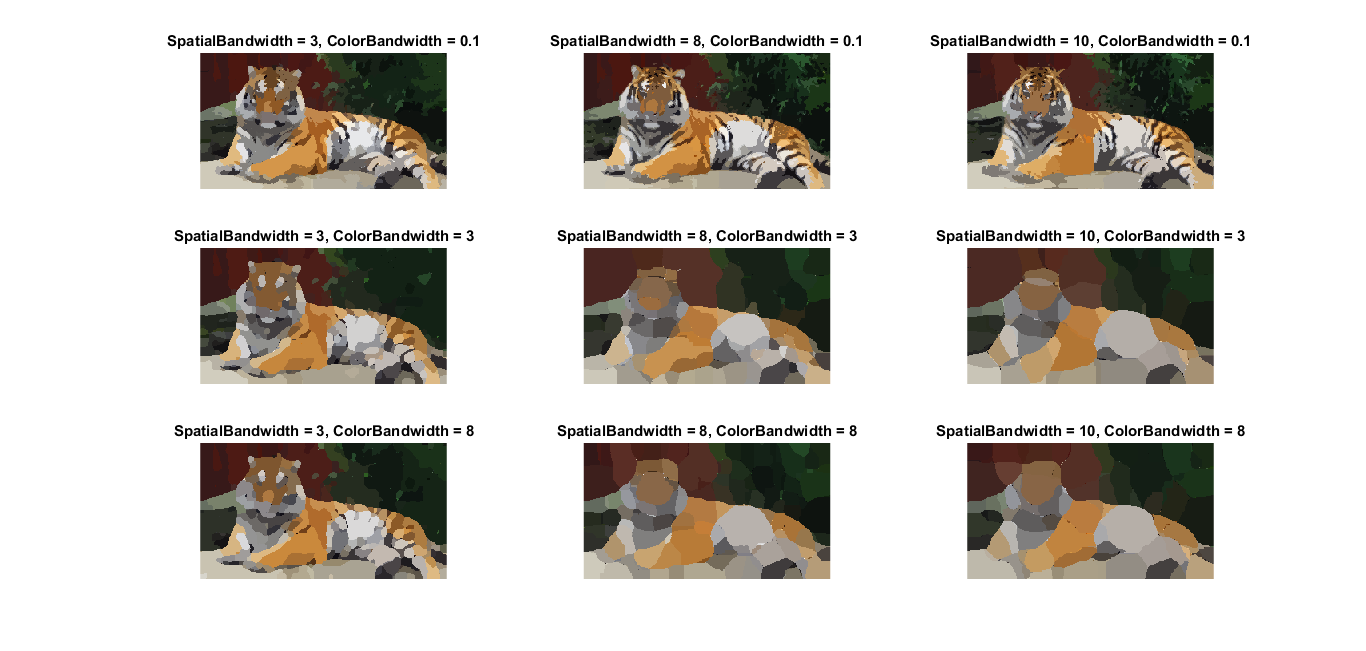
\includegraphics[width=1.2\linewidth]{meanshift.png}
        \caption{Result of meanshift}
        \label{fig:5}
    \end{figure}
    
    \item %Q6
    \textbf{What kind of similarities and differences do you see between K-means and mean-shift segmentation?}
    \par
    Mean-shift segmentation is a non-parametric approach, except by the hyperparameter (bandwidth) in the kernel definition. This means the mean-shift algorithm segments the image by assigning each sample point to a mode, without however actually estimating the whole probability density function that generated the samples. K-means, however, implicitly models the probability density as a superposition of spherically symmetric distributions - but it still does not require any probabilistic modeling. This all means that, differently from k-means, mean-shift segmentation doesn't require pre-determining the number of clusters, which is great. Additionally, in the case of this assignment, we are aggregating positional information to the features in mean-shift segmentation, while only using information about color in the k-means algorithm.
    
    It can be said that both algorithms make use of clustering to find regions that are somewhat similar in the image.
    
\section{Normalized Cut}

    \item %Q7
    \textbf{Does the ideal parameter setting vary depending on the images? If you look at the images, can you see a reason why the ideal settings might differ?}
    \par
    
    Yes, as expected. The number of objects are different in different images (which may affect the maximum depth), the formats of the segments differ as well (which may affect the radius), the difference in colors (background x foreground) also differ (which may affect the color bandwidth). Figure \ref{figNormCuts1} shows the result of applying NormCuts in the image tiger1.
    
    \begin{figure}[H]
        \centering
        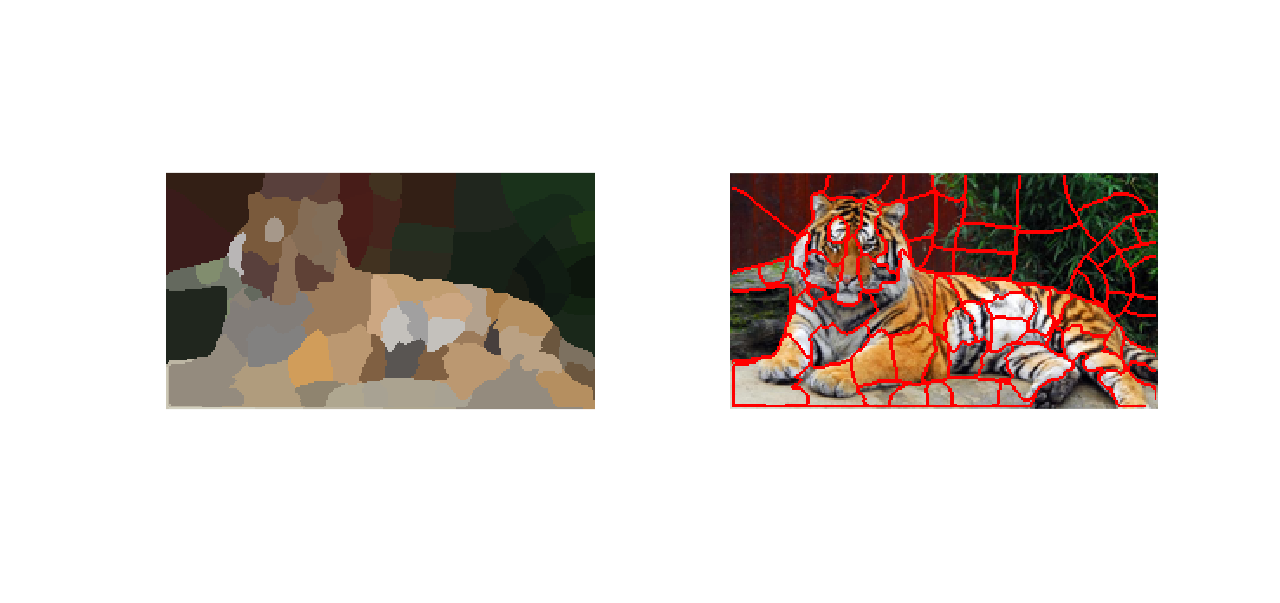
\includegraphics[width=1.2\linewidth]{normcuts1.png}
        \caption{NormCuts: colour_{bandwidth} = 20; radius = 3; ncuts_{thresh} = 0.2; min_{area} = 50; max_{depth} = 6}
        \label{figNormCuts1}
    \end{figure}
    
    \item %Q8
    \textbf{Which parameter(s) was most effective for reducing the subdivision and still result in a satisfactory segmentation?}
    \par
    
    The parameters $ncuts_{thresh}$ and $min_{area}$ were most useful to reduce the subdivision and still result in a satisfactory segmentation. Figures \ref{figNormCuts2} and \ref{figNormCuts3} show the results.
    
    \begin{figure}[H]
        \centering
        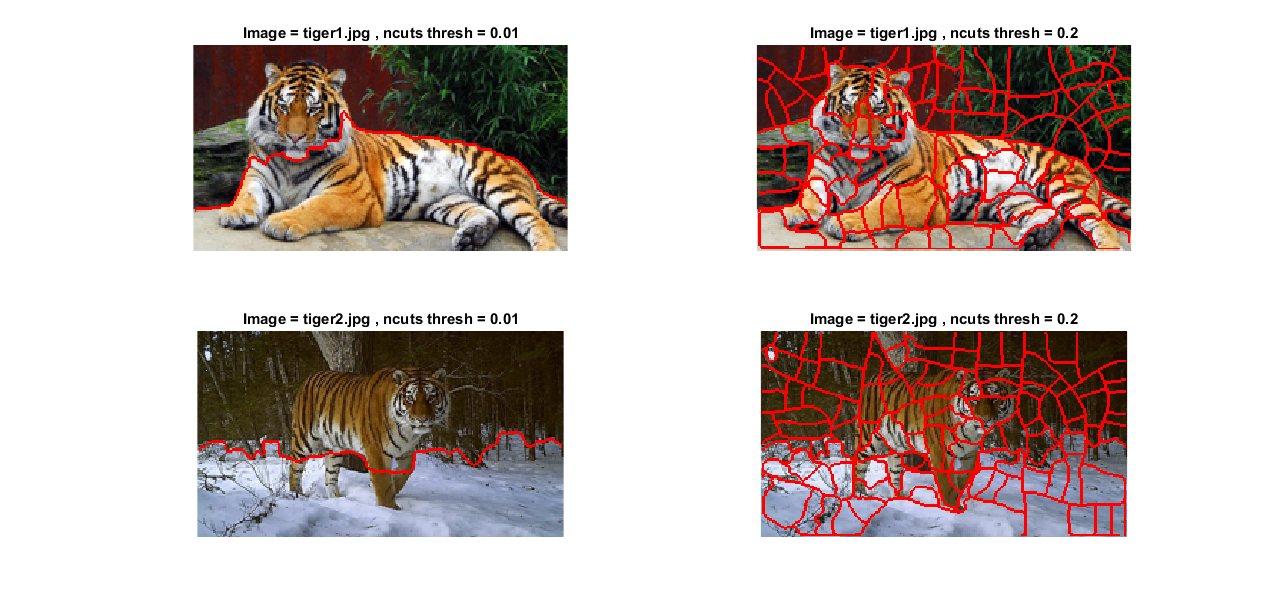
\includegraphics[width=1.2\linewidth]{normcuts2.png}
        \caption{NormCuts: colour_{bandwidth} = 20; radius = 3; ncuts_{thresh} = 0.01 and 0.2; min_{area} = 200; max_{depth} = 8}
        \label{figNormCuts2}
    \end{figure}
    
    \begin{figure}[H]
        \centering
        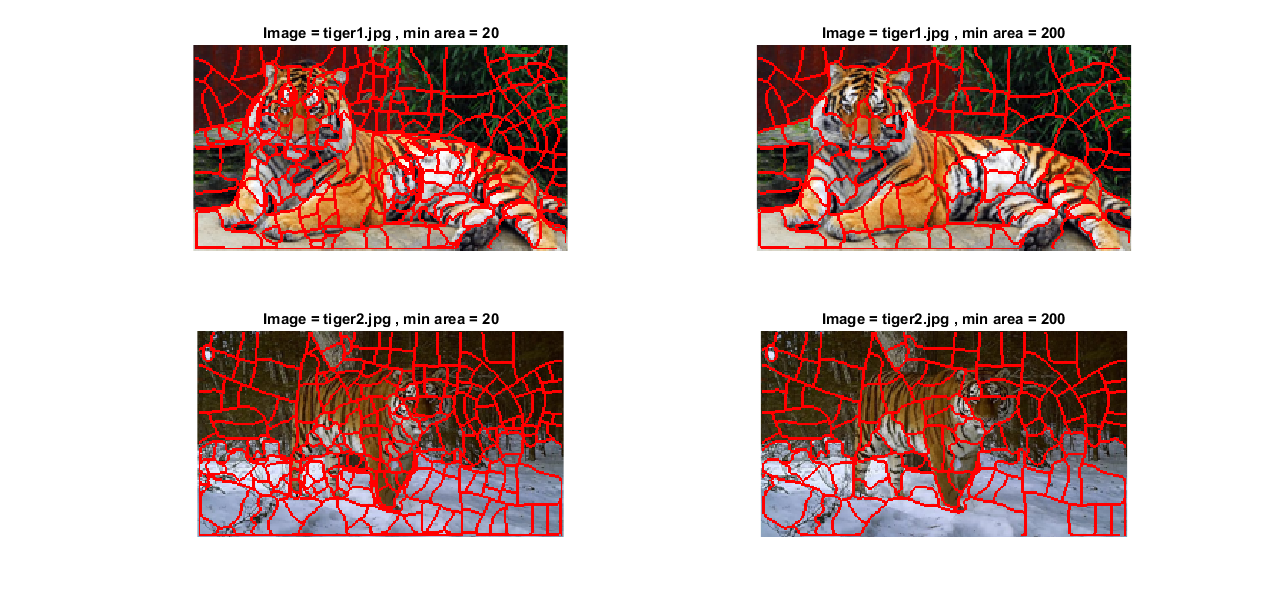
\includegraphics[width=1.2\linewidth]{normcuts3.png}
        \caption{NormCuts: colour_{bandwidth} = 20; radius = 3; ncuts_{thresh} = 0.2; min_{area} = 20 and 200; max_{depth} = 8}
        \label{figNormCuts3}
    \end{figure}

    \item %Q9
    \textbf{Why does Normalized Cut prefer cuts of approximately equal size? Does this happen in practice?}
    \par
    
    Because the objective function itself induces the areas to be more or less of the same size. Yes, this can be observed in practice, via the given figures.
    
    \item %Q10
    \textbf{Did you manage to increase radius and how did it affect the results?}
    
    It makes the contours follow the true edges better, which was expected. Figure \ref{figNormCuts4} shows the difference.
    
    \begin{figure}[H]
        \centering
        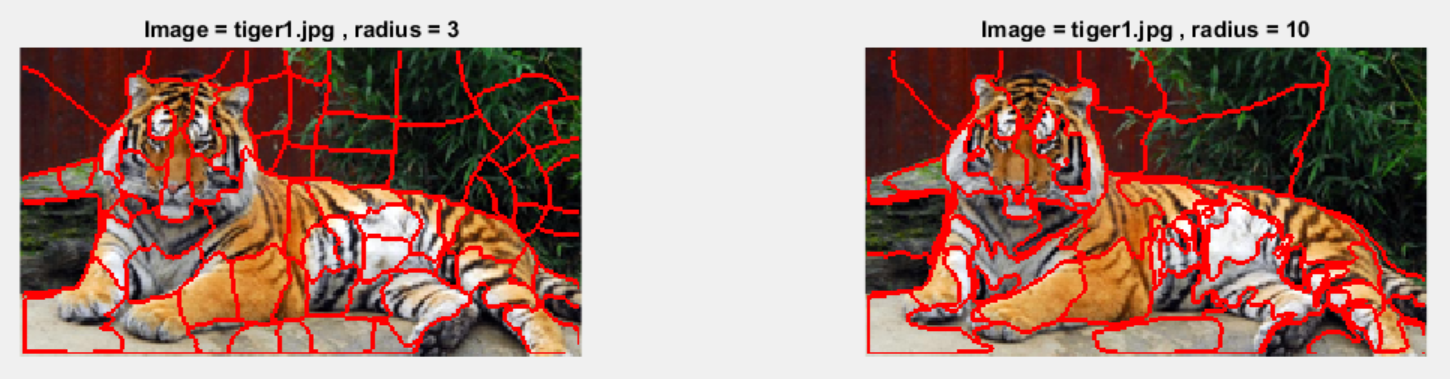
\includegraphics[width=1.2\linewidth]{normcuts4.png}
        \caption{NormCuts: colour_{bandwidth} = 20; radius = 3 and 10; ncuts_{thresh} = 0.2; min_{area} = 50; max_{depth} = 6}
        \label{figNormCuts4}
    \end{figure}
    
\section{Segmentation using graph cuts}

    \item %Q11
    \textbf{Does the ideal choice of \textit{alpha} and \textit{sigma} vary a lot between different images?}
    \begin{enumerate}
    \item orange : Not very sensible to the parameter since the shape is not very complex. $alpha = 4$ and $sigma = 6$ seems to be fine.
        \begin{figure}[H]
        \centering
        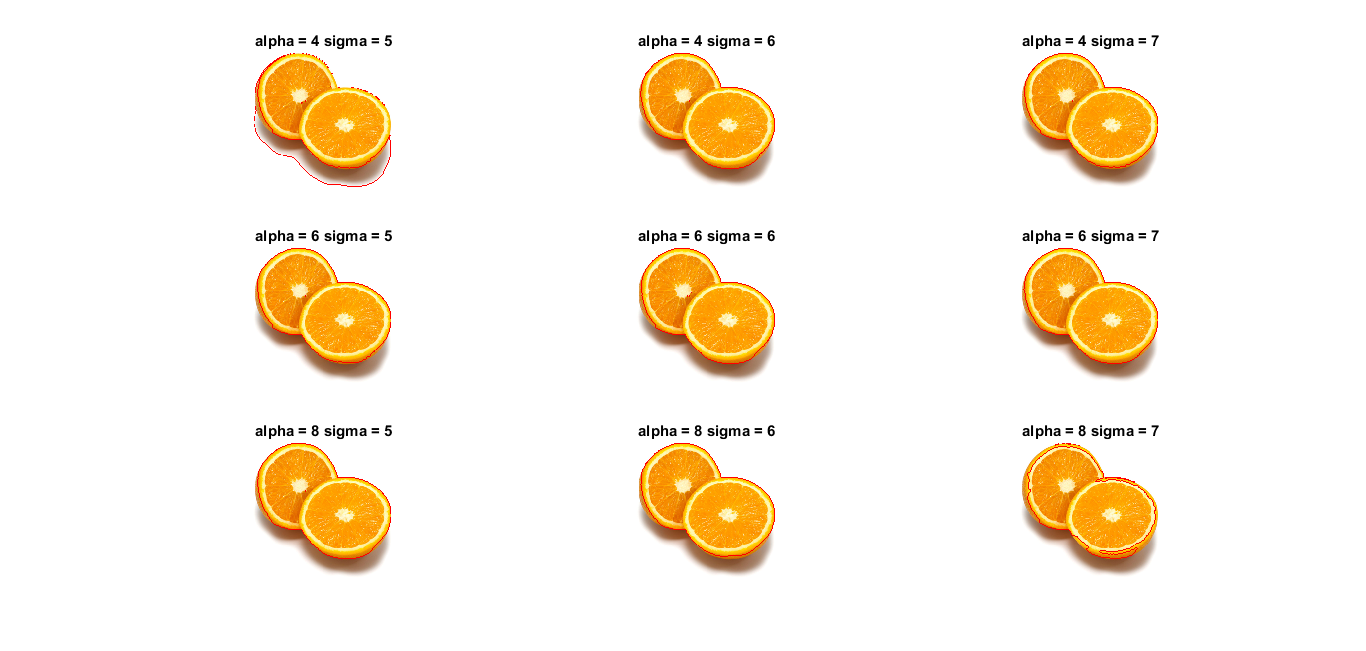
\includegraphics[width=1.2\linewidth]{graphcut_sigma_alpha0.png}
        \caption{Results with different $\alpha$ and $\sigma$ for \textit{orange.jpg}}
        \label{fig:5110}
    \end{figure}
    
    
    \item tiger1 : $alpha = 8$ and $sigma = 10$
        \begin{figure}[H]
        \centering
        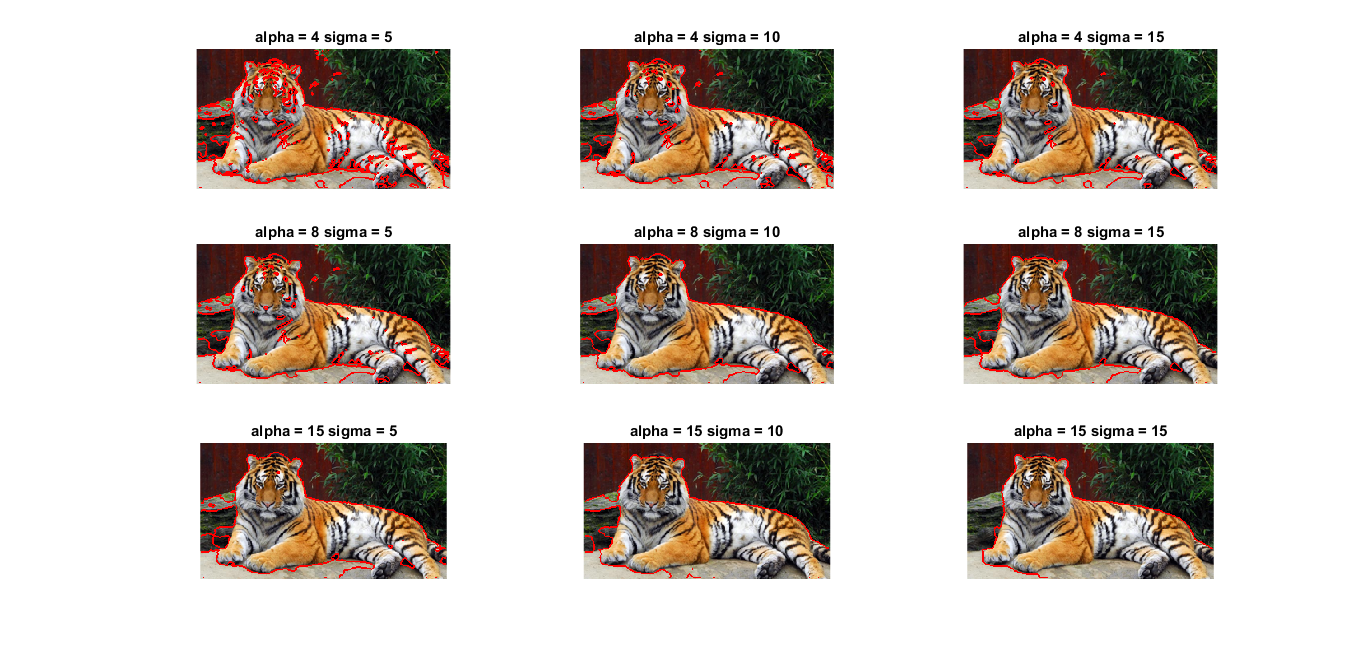
\includegraphics[width=1.2\linewidth]{graphcut_sigma_alpha1.png}
        \caption{Results with different $\alpha$ and $\sigma$ for \textit{tiger1.jpg}}
        \label{fig:5111}
    \end{figure}
    
    \item tiger2 : hard to find the optimal. $alpha = 15$ and $sigma = 10$ seems to be OK.
        \begin{figure}[H]
        \centering
        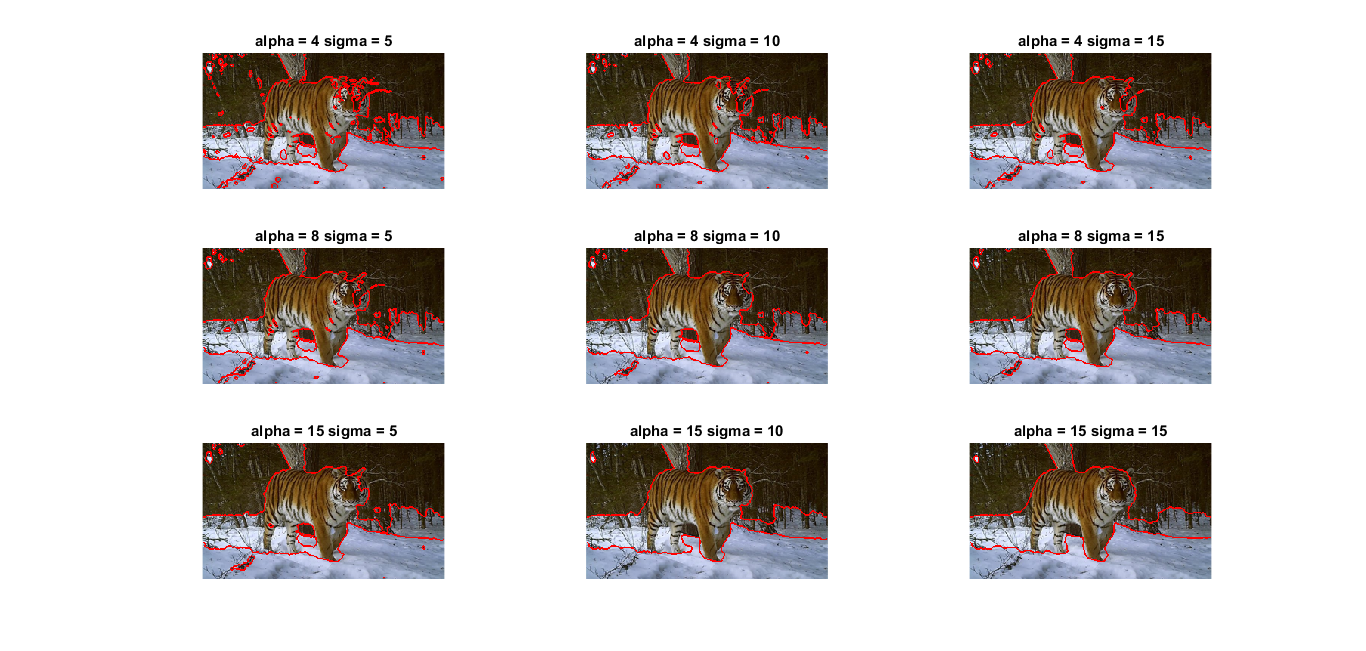
\includegraphics[width=1.2\linewidth]{graphcut_sigma_alpha2.png}
        \caption{Results with different $\alpha$ and $\sigma$ for \textit{tiger2.jpg}}
        \label{fig:5112}
    \end{figure}
    
    \item tiger3 : $alpha = 15$ and $sigma = 15$ seems to be optimal.
        \begin{figure}[H]
        \centering
        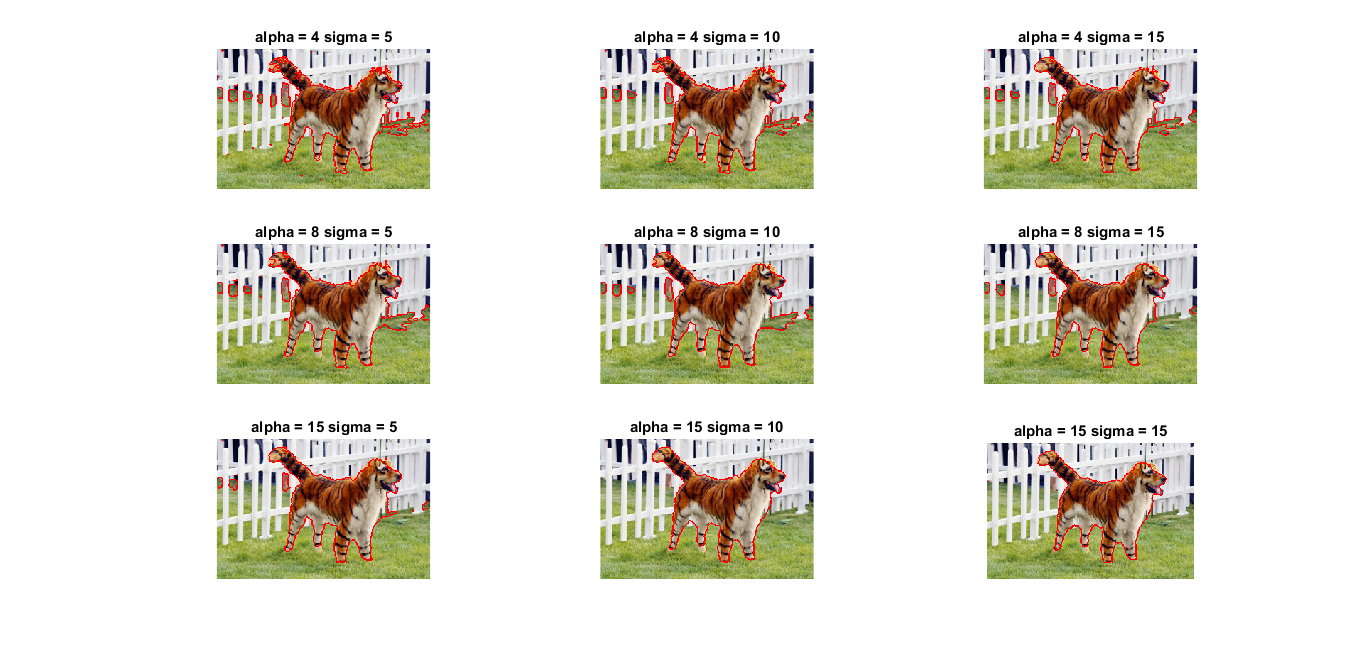
\includegraphics[width=1.2\linewidth]{graphcut_sigma_alpha3.png}
        \caption{Results with different $\alpha$ and $\sigma$ for \textit{tiger2.jpg}}
        \label{fig:5113}
    \end{figure}
    
    \end{enumerate}
    
    \item %Q12
    \textbf{How much can you lower K until the results get considerably worse?}
    \par
    $K = 6$ is still generates acceptable result for $tiger1.jpg$, as shown in Figure \ref{fig:5121}.
   \begin{figure}[H]
        \centering
        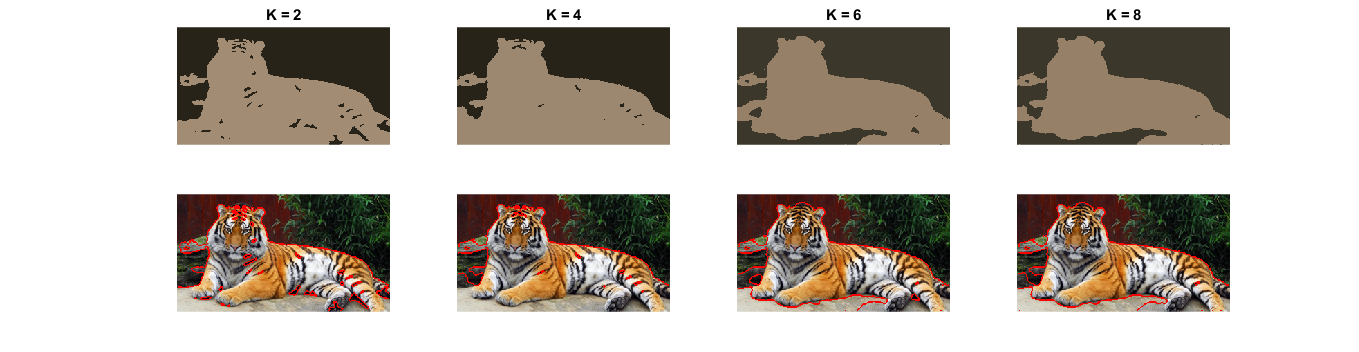
\includegraphics[width=1.2\linewidth]{graphcut_K1.png}
        \caption{Results with different K for \textit{tiger1.jpg}}
        \label{fig:5121}
    \end{figure}  
    \par $K = 2$ is still generates acceptable result for $tiger3.jpg$, 
    
    \begin{figure}[H]
        \centering
        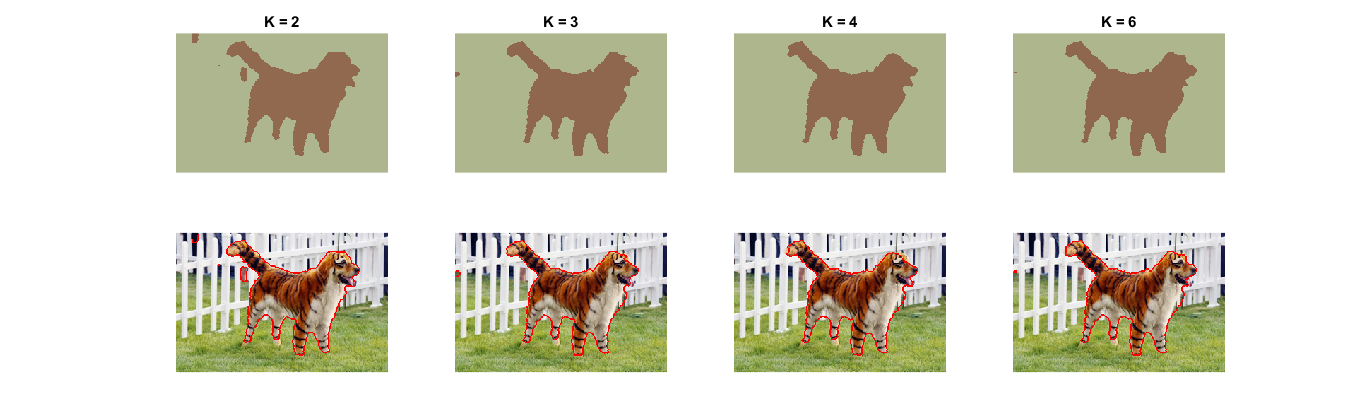
\includegraphics[width=1.2\linewidth]{graphcut_K3.png}
        \caption{Results with different K for \textit{tiger3.jpg}}
        \label{fig:5122}
    \end{figure}  
    
    
    \item %Q13
    \textbf{Unlike the earlier method Graph Cut segmentation relies on some input
from a user for defining a rectangle. Is the benefit you get of this worth the effort?
Motivate!}
\par
    Yes, the results of different initialization area is shown as below:
    \begin{figure}[H]
        \centering
        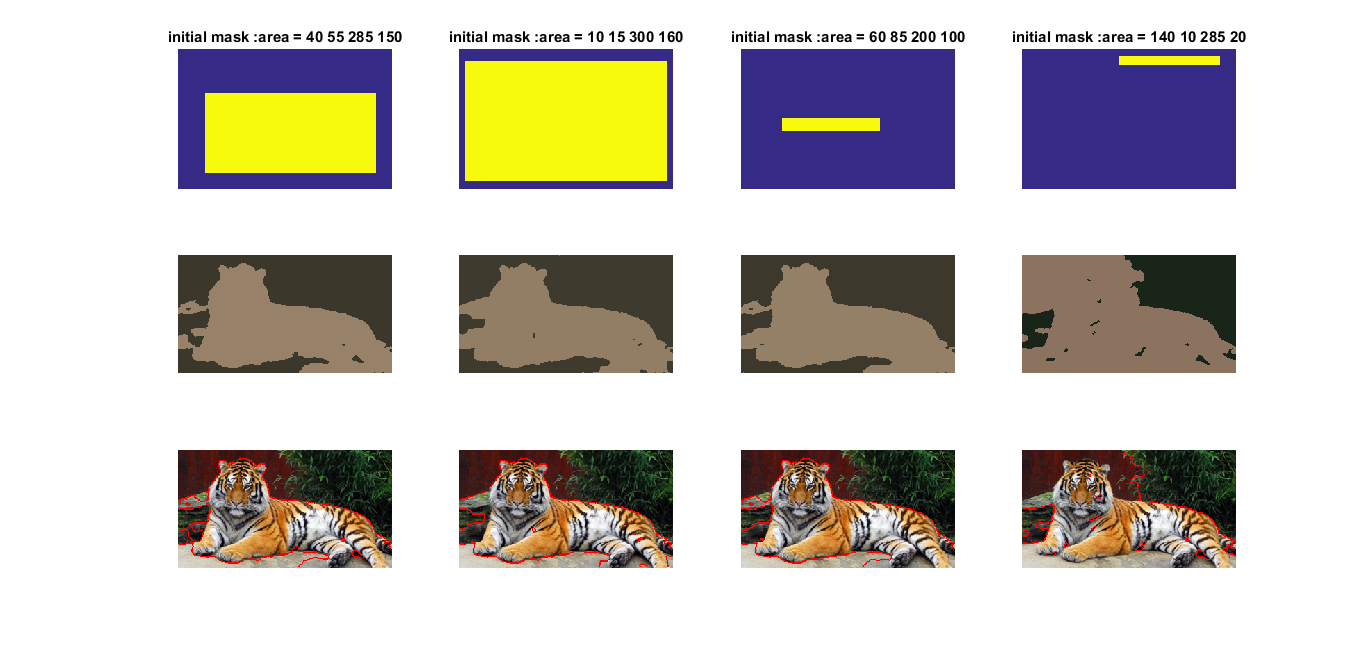
\includegraphics[width=1.2\linewidth]{graphcut_initialarea.png}
        \caption{Results with different initialization}
        \label{fig:513}
    \end{figure}
    The initial rectangle gives the prior knowledge on the foreground and background. If the initialization is too large, it will include more pixels into foreground in the end and if too biased it will lead to converging to wrong object as foreground.
    
    \item %Q14
    \textbf{What are the key differences and similarities between the segmentation
methods (K-means, mean-shift, Normalized Cut and energy-based segmentation with
Graph Cuts) in this lab? Think carefully!!}
%The first three only take segments, but the last consider foreground and background as well.

The K-means and graph-cut have very similar approaches in the sense that they associate pixels to a class. However graph-cut makes use of a smooth association, while k-means makes use of a harsh association.

Both K-means and mean-shift take averages in order to find the segmentations. The graph-cut also takes a similar approach.

Normalized Cut and Graph-cut are graph-based methods. Mean-shift takes a "non-parametric" method to find the segments, while graph-cut takes a parametric method.



\end{enumerate}
\end{document}
